%Fancy RCS footer:
     \fancyfoot[C]{\texttt{1\_grupe.tex}}
     \fancyfoot[RO,LE]{\mbox{$$Revision: 1.7 $$}}
     \fancyfoot[LO,RE]{\mbox{$$Date: 2011-09-21 $$}}
% Correcting the title chapter page
\fancypagestyle{plain}{%
    \fancyhf{}
    \fancyhead[RO,LE]{\bfseries \thepage}
    \fancyhead[CO]{\rightmark}
    \fancyhead[CE]{\leftmark}
     \fancyfoot[C]{\texttt{1\_grupe.tex}}
     \fancyfoot[RO,LE]{\mbox{$$Revision: 1.7 $$}}
     \fancyfoot[LO,RE]{\mbox{$$Date: 2011-09-21 $$}}
    \renewcommand{\headrulewidth}{0.4pt}
    \renewcommand{\footrulewidth}{0.4pt}}

\chapter{Grupe - opći pojmovi}

\section{Definicija grupe i primjeri}

Vidi na str. \pageref{id:5}

\begin{definicija}[Grupa] 
Grupa $(G,\circ)$ je skup objekata $G$ na kojem je definirana binarna operacija
 $\circ$ tako da su zadovoljena slijedeća svojstva:
\begin{enumerate}[1)]
\item Zatvorenost: $g_1, g_2 \in G \imp g_1 \circ g_2 \in G$
\item Asocijativnost: $ g_1 \circ (g_2 \circ g_3) =
                       (g_1 \circ  g_2)\circ g_3$
\item Egzistencija identiteta: 
    $\exists e \td g\circ e = e \circ g = g \quad \forall g\in G$
\item Egzistencija inverza: 
  $\forall g\in G \;\; \exists g^{-1} \td g\circ g^{-1} = g^{-1}\circ
g =e$
\end{enumerate}
\end{definicija}


\begin{primjer}[$\mathbb{Z}$, +]
 Lako se uvjeriti da skup cijelih brojeva $\mathbb{Z}$ čini grupu obzirom
 na obično zbrajanje brojeva:
\begin{enumerate}[1)]
\item $n,m \in  \mathbb{Z} \imp n+m \in  \mathbb{Z}$
\item n+(m+k)=(n+m)+k
\item 0+n=n \quad \text{nula je identitet tj. ``jedinični element''}
\item n+(-n)=0
\end{enumerate}
\end{primjer}

\begin{primjer}[$\mathbb{Z}$, $\cdot$]
S druge strane, taj isti skup $\mathbb{Z}$ nije grupa obzirom na
operaciju množenja. Zašto? \secret{Nema inverza.}
\end{primjer}

\begin{primjer}
Skup dvije matrice
\[\left\{
\begin{pmatrix}
1 & 0 \\ 0 & 1
\end{pmatrix}, \;
\begin{pmatrix}
0 & 1 \\ 1 & 0
\end{pmatrix}
\right\} \]
čini grupu obzirom na uobičajeno množenje matrica. Promotrimo li pak skup
\emph{svih} $2\times2$ matrica vidimo da on \emph{ne} čini grupu jer nije
zadovoljen aksiom egzistencije inverza. Naime, neregularne matrice (one
čija determinanta iščezava) nisu invertibilne. Međutim, ukoliko se
ograničimo samo na skup regularnih  $2\times2$ matrica dobivamo grupu
koja se naziva \emph{opća linearna grupa} u dvije dimenzije i označava
grupno-teorijskom oznakom GL(2).
\end{primjer}

Grupu zovemo \emph{Abelova (abelovska, komutativna)} ako 
$\forall g_1, g_2 \in G \quad g_1 \circ g_2 = g_2 \circ g_1$

Npr. ($\mathbb{Z}$, +) je Abelova dok grupa GL(2) to nije.

Broj elemenata grupe nazivamo \emph{red grupe}. Obzirom na njega razlikujemo:
\begin{itemize}
\item \emph{Konačne grupe}. Primjer: ($\{1,-1\}$, $\cdot$)
\item \emph{Beskonačne diskretne grupe} koje imaju 
prebrojivo\footnote{Beskonačan skup je \emph{prebrojiv} ukoliko je moguće uspostaviti
bijektivno preslikavanje između tog skupa i skupa prirodnih brojeva $\mathbb{N}$. Npr. skup
racionalnih brojeva $\mathbb{Q}$ jest prebrojiv, dok skup realnih brojeva
$\mathbb{R}$ to nije.}
beskonačan broj elemenata. Primjer: ($\mathbb{Z}$, +)
\item \emph{Beskonačne kontinuirane grupe} 
koje imaju neprebrojiv broj elemenata i čije elemente možemo
zamisliti kao kontinuirani skup točaka. Ukoliko su zadovoljeni neki dodatni
uvjeti, vidi Poglavlje \ref{chap:lie}, ove grupe se nazivaju Lieve grupe. 
Primjeri: ($\mathbb{R}\backslash\{0\}$, $\cdot$), GL(2)
\end{itemize}

\begin{primjer}[Grupa simetrija]
Skup svih transformacija simetrije tj. transformacija koje ostavljaju
neki objekt nepromijenjen nužno tvore grupu.

\begin{enumerate}[1)]
\item zatvorenost: ako ni $g_1$ ni $g_2$ ne mijenjaju objekt, ne mijenja
   ga ni $g_2 \circ g_1$

\item asocijativnost je očita (zapravo, nije baš, čini se \dots)

\item identiteta - transformacija koja ne radi ništa ne mijenja objekt
   po definiciji

\item suprotna transformacija je isto simetrija
\end{enumerate}

``Objekt'' na kojeg djeluju transformacije grupe simetrija može biti
nekakav realan fizikalni objekt poput kristala, ali može biti i
nešto apstraktniji entitet poput kvantnomehaničke valne funkcije.

Važno je imati na umu da su sam pojam i svojstva grupe neovisni o
tom objektu. Njega ćemo iskoristiti da identificiramo skup transformacija
simetrije, da vizualiziramo pojedine transformacije i da
fizikalno interpretiramo rezultate teorije grupa, ali nikad
ne smijemo izgubiti iz vida da je grupa sasvim apstraktan matematički pojam.

\end{primjer}


\begin{primjer}[Ciklička grupa C$_n$]
Ciklička grupa C$_n$ je grupa simetrija rotacija pravilnog poligona s $n$
usmjerenih stranica.

\centerline{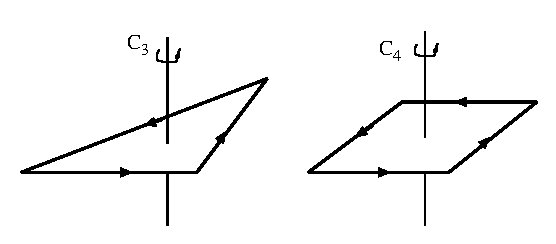
\includegraphics[scale=1.0]{pics/Cn}}

Elementi grupe C$_n$ su rotacije za kuteve 2$\pi r/n$, ($r=0,1,\ldots, n-1$)
oko osi koja okomito probada središte poligona. Usmjerenost
stranica isključuje rotacije oko osi koje leže u ravnini poligona. 
(Iako je poligon ravninski lik ovdje ga zamišljamo u 3D prostoru.)

Specifično svojstvo cikličkih grupa je da je sve elemente grupe moguće
dobiti uzastopnim množenjem jednog od njih sa samim sobom.
Tako npr. uzastopnim množenjem rotacije za kut 2$\pi/3$ sa samom sobom dobivamo ostale
dvije rotacije koje sačinjavaju grupu C$_3$: rotaciju za 4$\pi/3$ i
rotaciju za 0 radijana. 
Ukoliko označimo ``generirajuću'' rotaciju grupe C$_n$ (onu za kut 2$\pi/n$) simbolom 
$c$ onda možemo pisati
\begin{equation}
 \text{C}_n = \{c,c^2, \ldots , c^n=e \}
\label{eq:cn}
\end{equation}
odnosno grupu C$_n$ možemo alternativno definirati kao grupu generiranu
elementom $c$ sa svojstvom $c^n=e$ i pisati kao definicioni izraz:
\begin{equation}
 {\rm C}_n = {\rm gp}(c) \;, \qquad c^n=e \;.
\label{eq:cngp}
\end{equation}

Treću mogućnost za definiciju ove i drugih grupa pruža nam grupna tablica množenja
(poznata i kao Cayleyjeva tablica).
Naime, obzirom da je apstraktna grupa potpuno određena time da se navede
skup elemenata koji je sačinjavaju te time da se potpuno specificira kako
se ti elementi množe (tj. kakva je binarna operacija u grupi), grupu C$_3$, npr.,
je moguće definirati naprosto kao grupu koja zadovoljava slijedeću tablicu
množenja:

\begin{equation}
\begin{array}{c|ccc}
g_1\backslash\ g_2 & e & c & c^2 \\ \hline
   e    & e & c & c^2 \\
   c    & c & c^2 & e \\
   c^2    & c^2 & e & c
\end{array}
\label{eq:cntab}
\end{equation}

Grupne tablice množenja zadovoljavaju tzv. svojstvo latinskog
kvadrata poznato i kao
\begin{teorem}[Teorem o razmještaju]
Svaki element grupe se pojavljuje jednom i samo jednom u svakom stupcu
ili retku grupne tablice množenja.
\end{teorem}

\emph{Dokaz}: Zamislimo suprotno tj. da se u nekom retku
dvaput pojavi isti element, recimo $a$. To znači da je $a$ moguće
dobiti množenjem prvog elementa iz tog retka, neka je to $k$, s
dvama različitim elementima, recimo $m$ i $n$: $km=a$ i $kn=a$. To bi značilo
da je $km=kn$, a egzistencija inverza omogućuje ``skraćivanje''
ovakvih relacija tj. množenje slijeva s $k^{-1}$ pa
dobivamo $m=n$ što je kontradiktorno jer smo pretpostavili da su
$m$ i $n$ različiti elementi. Slično bi bilo za ponavljanje istog
elementa dvaput u istom stupcu.

Treba uočiti da nam binarna operacija definirana tablicom množenja
koja je u standardnom obliku gdje prvi redak i stupac odgovaraju
jediničnom elementu i koja poštuje teorem o razmještaju automatski 
garantira zadovoljavanje tri aksioma grupe: 
\emph{zatvorenost} (u tablici se pojavljuju samo elementi grupe), 
\emph{egzistencija identiteta} (po konstrukciji prvog retka i stupca) i
\emph{egzistencija inverza} (u svakom retku se nužno pojavljuje i 
jedinični element i odgovarajući stupac je onda stupac inverza).
Međutim, svojstvo \emph{asocijativnosti} nije nužno zadovoljeno
i treba ga provjeriti nekim drugim načinom\footnote{Eksplicitna provjera
može biti mukotrpna. Od pomoći je procedura poznata kao Lightov
test asocijativnosti.}.


Ove dvije alternativne definicije (\ref{eq:cngp}) i (\ref{eq:cntab}) 
naglašavaju apstraktnu prirodu grupe (ne treba
nam trokut kao objekt grupe simetrija).

Inače, C$_n$, za $n=2,3,4,6$ spada u kristalografske \emph{točkaste grupe} kakvih
ima ukupno 32\footnote{U 3D prostoru. U 2D prostoru postoji 10, a u
1D prostoru samo dvije točkaste grupe.}. 
To su grupe prostornih simetrija savršenih beskonačnih
periodičnih kristala koje ostavljaju jednu točku nepomičnom. (Za
razliku od npr. translacije za konstantu rešetke koja je isto simetrija
kristala, ali nijednu točku ne ostavlja na mjestu.)
  
Može se pokazati da jedini elementi tih grupa mogu biti kompozicije
rotacija za 60$^\circ$ i 90$^\circ$ te inverzije $\vec{r}\to -\vec{r}$.
(cf. Crystallographic restriction theorem)
   
\end{primjer}



\begin{primjer}[Dihedralna grupa D$_n$]
Dihedralna grupa D$_n$ je grupa simetrija rotacija pravilnog poligona s $n$ stranica.
Prma slici

\centerline{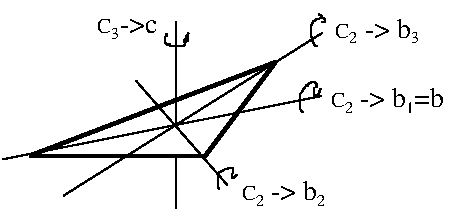
\includegraphics[scale=1.0]{pics/D3}}

elementi grupe su rotacije $e, c$ i  $c^2$ baš kao kod grupe C$_n$, te
dodatno rotacije $b_1, b_2$ i $b_3$ za kut $\pi$ oko triju horizontalnih
osi.

Uočimo sada neka svojstva množenja u toj grupi. Kao prvo, vrijedi
da je $b_2 = c b_1 c^{-1}$ tj. da su $b_2$ i $b_1$ međusobno
\emph{konjugirani} preko elementa $c$. Da je to tako vidi
se iz slike:

\centerline{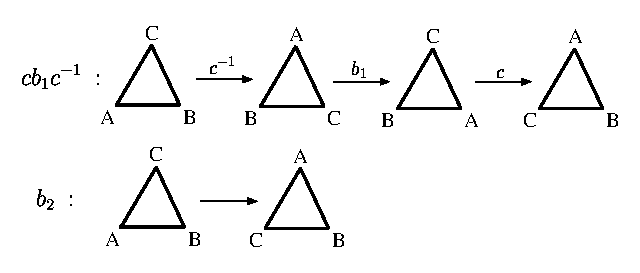
\includegraphics[scale=1.0]{pics/cbc}}

Na sličan način se možemo uvjeriti da je $b_2 = b_1 c $
i $b_3 = b_1 c^2 $, odnosno da 
$c$ i $b\equiv b_1$ generiraju sve ostale transformacije
\begin{equation}
{\rm D}_3=\{e,c,c^2,b,bc,bc^2\} \;.
\label{eq:d3el}
\end{equation}
To sugerira da bismo grupu D$_3$ mogli definirati kao
\begin{equation}
 {\rm D}_3={\rm gp}(c, b) \;, \qquad c^3 = b^2 = e  \;,
\label{eq:d3gp1}
\end{equation}
no ova definicija nije kompletna jer nam nedostaje još
i pravilo za komutiranje elemenata (koje nam nije trebalo
za grupu C$_n$ koja je Abelova). Njega dobijemo tako da
iskombiniramo dvije gore dobivene relacije: 
$b_2 = c b_1 c^{-1} = b c$ i pomnožimo zdesna s $c$:
\begin{equation}
c b = b c^2
\label{eq:d3com}
\end{equation}
Ova relacija sad omogućuje da proizvoljan umnožak elemenata
grupe (npr. $b c b^2 c^5 b$ svedemo na oblik $b^\alpha c^\beta$ gdje
je $\alpha<2$ i $\beta<3$, tj. na jedan od elemenata iz (\ref{eq:d3el}).
Za kompaktan zapis definicije grupe D$_3$ koji će se onda moći
lako generalizirati i na ostale D$_n$ grupe, množimo gornju
komutacijsku relaciju (\ref{eq:d3com}) slijeva s $b$ i zdesna s $c$
i dobivamo  $ bcbc \equiv (bc)^2 = b^2 c^3 = e$ pa možemo
pisati
\begin{equation}
 {\rm D}_3={\rm gp}(c,b) \;, \qquad c^3 = b^2 = (bc)^2 = e
\label{eq:d3gp}
\end{equation}
Ova definicija se generalizira ovako (vidi zadatke)
\begin{equation}
 {\rm D}_n={\rm gp}(c,b) \;, \qquad c^n = b^2 = (bc)^2 = e
\label{eq:dngp}
\end{equation}
što onda možemo iskoristiti i da bismo definirali grupu
D$_2$ poznatu i kao
\emph{Kleinova četvorna grupa} (njem. \emph{Vierergruppe}), 
za koju nemamo odgovarajući poligon kao objekt grupe simetrija.
\end{primjer}


\section{Podgrupe}

\begin{definicija}[Podgrupa]
Podgrupa $H$ grupe $G$ je neprazni podskup $H\subset G$ koji i sam
tvori grupu obzirom na grupnu operaciju definiranu na $G$.
Podgrupu $H\neq\{e\}\neq G$ zovemo \emph{prava} podgrupa i pišemo $H<G$.
\end{definicija}

\begin{primjer}
C$_2$=\{e, b\} i C$_3$=\{e, c, c$^2$\} su prave podgrupe od D$_3$
\end{primjer}

\begin{primjer}
Grupa translacija i točkasta grupa su podgrupe grupe prostornih
simetrija kristala.
\end{primjer}

\begin{definicija}[Susjedna klasa]
Lijeva susjedna klasa (engl. coset) podgrupe $H$ obzirom na element
$g\in G$ je skup
\begin{displaymath}
     gH=\{gh \td h\in H\}
\end{displaymath}
\end{definicija}

Odnos pripadnosti elementa $g_1$ lijevoj susjednoj klasi obzirom na element $g_2$,  
$g_1 \in g_2 H$, uspostavlja \emph{relaciju ekvivalencije}%
\footnote{Općenito, \emph{relacija ekvivalencije} je binarna relacija $a\sim b$ između
elemenata nekog
skupa koja ima slijedeća svojstva
\begin{enumerate}[(i)]
\item $a\sim a \quad \forall a$ \qquad (refleksivnost)
\item $a\sim b \imp b\sim a$   \qquad (simetričnost)
\item $a\sim b \quad \textrm{i}\quad  b\sim c \imp a\sim c$  \qquad (tranzitivnost)
\end{enumerate}
Primjeri relacija ekvivalencije su: ``osoba $a$ je rođena na isti dan kad i osoba $b$''
ili ``trokut $a$ je sličan trokutu $b$'', dok npr. ``broj $a$ je veći ili jednak
broju $b$'' nije relacija ekvivalencije jer nije simetrična.
(Ona je antisimetrična. Binarna relacija na skupu koja je refleksivna, antisimetrična
i tranzitivna zove se \emph{relacija uređaja}.)
Svaka relacija ekvivalencije cijepa skup na disjunktne \emph{klase ekvivalencije}.
} između ta dva elementa u grupi G, $g_1 \sim g_2$.

Susjedne klase po nekoj podgrupi $H$ su međusobno disjunktne i
sve imaju isti broj elemenata (jednak redu od $H$, zahvaljujući
Teoremu o razmještaju) pa tako
definiraju jednu particiju grupe G:

\centerline{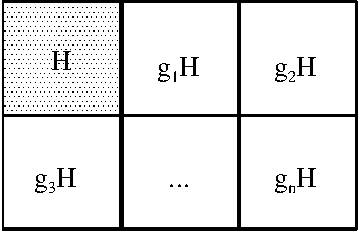
\includegraphics[scale=1.0]{pics/lagrange}}

Promatrajući ovu sliku lako se uvjerimo u točnost Lagrangeovog
teorema:

\begin{teorem}[Lagrange]
Red podgrupe dijeli red grupe.
\end{teorem}

\begin{definicija}[Kvocijentni skup]
Skup svih različitih lijevih susjednih klasa 
\begin{displaymath}
      G/H \equiv \{gH \td g\in G\}
\end{displaymath}
zove se \emph{lijevi kvocijentni skup grupe} $G$ po podgrupi $H$.
\end{definicija}

Potpuno analogno se definiraju desna susjedna klasa i desni kvocijentni
skup.

\begin{primjer}[D$_3$]
Promotrimo podgrupu $H=\{e, c, c^2\}=$C$_3$ grupe $G={\rm D}_3$.
Dvije lijeve susjedne klase su
\begin{enumerate}[1)]
\item $eH=H=\{e, c, c^2\}$ \; \text{i}
\item $bH=\{b, bc, bc^2\}$ \;,
\end{enumerate}
a kvocijentni skup je D$_3$/C$_3=\{eH, bH\}$. Postoji i kvocijentni 
skup D$_3$/C$_2$
\end{primjer}

\begin{definicija}[Normalna podgrupa]
Podgrupa za koju vrijedi $gH=Hg$, $\forall g\in G$, zovemo
\emph{normalna} ili \emph{invarijantna}.
\end{definicija}

\begin{primjer}[D$_3$]
$G=D_3$, $H=C_3$. $bC_3 = C_3 b$, \ldots (za ostale $g\in D_3$ trivijalno)
Dakle, $C_3$  je normalna podgrupa od $D_3$. S druge strane
$C_2 = \{e, b\}$ nije normalna jer npr. $c C_2 \neq C_2 c$.
\end{primjer}

Očito je da su za normalnu podgrupu $H$ lijevi i desni kvocijentni skupovi
identični  $G/H$ = $H\backslash$G

Grupe koje nemaju normalnih podgrupa zovu se \emph{jednostavne},
a one koje nemaju normalnih Abelovih podgrupa zovu se \emph{polujednostavne}.

Kvocijentni skup po normalnoj podgrupi čini grupu obzirom na
binarnu operaciju
\begin{displaymath}
       (g_1H)(g_2H)=(g_1 g_2)H
\end{displaymath}
Uvjerite se da su zadovoljeni aksiomi grupe.


\begin{primjer}[D$_{3}$/C$_3$]
Tablica množenja u ovom kvocijentnom skupu je definirana relacijama
\begin{align}
(eH)(eH) &= ee H = eH \\
(eH)(bH) &= bH  \\
(bH)(eH) &= bH  \\
(bH)(bH) &= eH 
\end{align}

Lijevi i desni kvocijentni skupovi su jednaki
\begin{align*}
{\rm D}_{3}/{\rm C}_3 &= \{\{e,c,c^2\}, \{b, bc, bc^2\}\} \\
{\rm C}_3\backslash{\rm D}_{3} &= \{\{e,c,c^2\}, \{b, cb=bc^2, c^2b=bc\}\}
    = D_{3}/C_3
\end{align*}
i imaju grupnu strukturu jednaku grupi C$_2$.

\end{primjer}

S druge strane
\begin{align*}
{\rm D}_{3}/{\rm C}_2 &= \{\{e,b\}, \{c, cb=bc^2\}, \{c^2, c^2b=bc\}\} \\
{\rm C}_2\backslash{\rm D}_{3} &= \{\{e,b\}, \{c, bc\}, \{c^2, bc^2\}\}
    \neq {\rm D}_{3}/{\rm C}_2
\end{align*}
i D$_{3}$/C$_2$ nije grupa.


\begin{definicija}[Konjugirani elementi]
Dva elementa $a$ i $b$ grupe $G$ su \emph{konjugirani} ukoliko
postoji $g\in G \td a=gbg^{-1}$.
\end{definicija}



Konjugacija je također relacija ekvivalencije:
\begin{enumerate}[(i)]

\item $a=e^{-1} a e  \imp a\sim a$
\item $a=g^{-1} b g  \imp  b= g^{-1} a (g^{-1})^{-1}$
\item $a=g b g^{-1}$, $b=hch^{-1}$, \\
         $a=ghch^{-1}g^{-1}=(gh)c(gh)^{-1}$, $gh\in G$
  
\end{enumerate}


Konjugacija (baš kao i svaka relacija ekvivalencije) definira
particiju skupa na klase.

\begin{displaymath}
   \text{klasa od $a$} = \{ b \td b=gag^{-1},\quad g\in G\}
\end{displaymath}

Klasa od $e=\{e\}$ što povlači da klase, izuzev ove trivijalne, nisu podgrupe.

Za Abelove grupe svaki element je klasa za sebe.

Normalne podgrupe zadovoljavaju $gHg^{-1}=H$, $\forall g\in G$. Slijedi
da su one sastavljenje od \emph{cijelih} klasa konjugacije.

\begin{primjer}[D$_3$]
Klase konjugacije  od D$_3$ su:
\begin{enumerate}[-]
\item $(e)$
\item $(c, c^{2})$
\item $(b, bc, bc^2)$
\end{enumerate}
i odgovaraju rotacijama za različite kuteve. Konjugirajući elementi
preslikavaju međusobno osi rotacije. Normalna podgrupa $C_3$ se
sastoji od cijelih klasa (prve dvije), dok podgrupa $C_2=\{e,b\}$ nema
to svojstvo i nije normalna.
\end{primjer}


\section{Homomorfizam i izomorfizam grupa}

\begin{definicija}[Homomorfizam]
Neka su $G$ i $H$ grupe, a $f:G\to H$ preslikavanje koje komutira
s grupnom operacijom tj. za koje vrijedi
\begin{displaymath}
      f(ab)=f(a)f(b) \quad \forall a,b\in G \;.
\end{displaymath}
Onda kažemo da je $f$ \emph{homomorfizam} grupe $G$ u grupu $H$.
\end{definicija}

Homomorfizam koji je i bijekcija zovemo \emph{izomorfizam} i
pišemo $A\cong B$ ili $A=B$.

Izomorfne grupe su s apstraktnog stanovišta jednake (imaju
istu tablicu množenja).

\begin{primjer}[C$_2$]
Grupa C$_2$ je izomorfna grupama $(\{1, -1\},\cdot$) i
$\left(\left\{
\begin{pmatrix}
1 & 0 \\ 0 & 1
\end{pmatrix},
\begin{pmatrix}
0 & 1 \\ 1 & 0
\end{pmatrix}
\right\},\cdot\right)$.
\end{primjer}

\emph{Slika} homomorfizma $f(A)$ (skup svih elemenata u $B$ koji imaju original u $A$) 
je podgrupa od $B$: $f(A)< B$ (DZ: Uvjerite se u to.)

\centerline{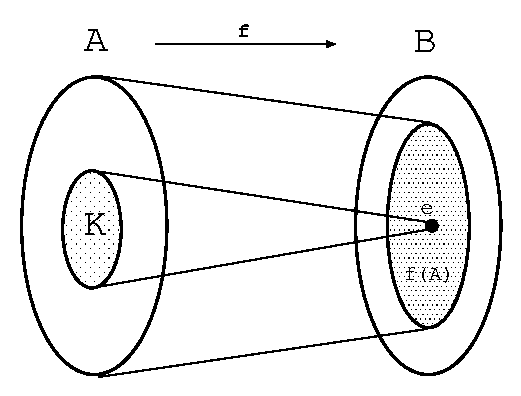
\includegraphics[scale=0.8]{pics/homomorfizam}}

Slika $f(e_A)$ jediničnog elementa $e_A$ iz $A$ je jedinični element $e_B$ u $B$ jer
množenjem relacije
$$ f(e_A) f(b) = f(e_A b) = f(b) $$
s desna s $f(b)^{-1}$ dobivamo
$$ f(e_A) = f(b) f(b)^{-1} = e_B \;. $$
No moguće je da se i drugi elementi iz $A$ osim jediničnog preslikavaju u 
jedinični element u $B$.
\emph{Kernel} homomorfizma je skup svih elemenata od $A$ koji se
preslikavaju u jedinični element iz $B$.
$$ K \equiv {\rm ker}(f) \equiv \{ k\in A \; | \; f(k) = e_B \} \;. $$

Kernel od $f:A\to B$ je normalna podgrupa od $A$. (DZ: Uvjerite se u to.)


\begin{teorem}[Teorem o izomorfizmu]
\label{th:izomorfizam}
Ako je $f:G\to G'$ homomorfizam s kernelom $K$, onda vrijedi
\begin{enumerate}[a)]
\item Svaki element susjedne klase $gK$ se preslikava u isti element $f(g)$.
\item Slika homomorfizma $f(G)$ je izomorfna kvocijentnoj grupi po kernelu $G/K$.
\end{enumerate}
\end{teorem}
(Skup $G/K$ je grupa jer je $K$ normalna podgrupa.)

Dokaz$^{*}$\secret{Cornwell '84, 2.6}: Pridruživanje je $f(g)\leftrightarrow gK$.
Pokažimo da je to pridruživanje dobro definirano i bijekcija te da čuva grupnu
strukturu.

- $f(g)\mapsto gK$ je dobro definirano jer je gK jedinstven: $f(g)=f(g')$
  $\imp f(g'g^{-1})=f(g')f(g^{-1})=f(g)f(g)^{-1}=e
   \imp g'g^{-1}\equiv k\in K, g'=kg \imp gK=g'K$
(Zadnja implikacija slijedi iz toga da $\forall k_1 \in K, gk_1 = 
g' k^{-1}k_1 \in g' K$)

\vspace*{1ex}

\centerline{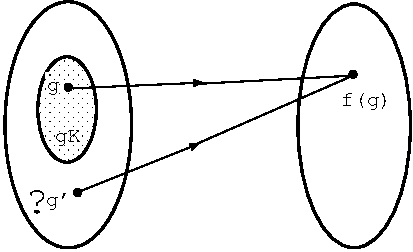
\includegraphics[scale=0.8]{pics/homo1}}

- $gK\mapsto f(g)$ je dobro definirano jer ne ovisi o izboru
  elementa $g$ iz $K$: $g,g'\in gK \imp g'g^{-1}\in K \imp
   \imp f(g'g^{-1})=e \imp f(g')f(g^{-1})=e \imp f(g')=f(g)$

\vspace*{1ex}

\centerline{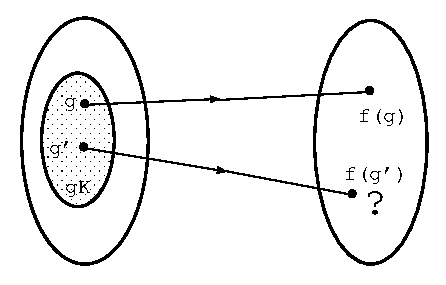
\includegraphics[scale=0.8]{pics/homo2}}

- injekcija u oba smjera $\imp$ bijekcija

- Čuvanje grupne strukture: f(g)f(g') se preslikava u (gK)(g'K) jer \\
  f(g)f(g')=f(gg')=gg'K=(gK)(g'K)
  
\vspace*{1ex}

\centerline{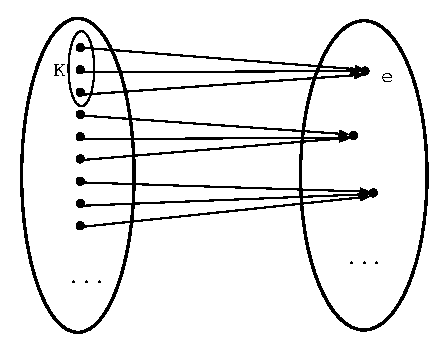
\includegraphics[scale=1.0]{pics/homo3}}

\secret{Primjer: $D_3$: $C_3\to e$, a ostali u $c$ iz $C_2$
 $\imp f(D_3) = C_2 = D_3/C_3$}

Jedan korolar ovog teorema je da je svaki element $g'$ iz $G'$ slika
istog broja elemenata iz G (zato jer susjedne klase moraju imati
isti broj elemenata). Drugi korolar je da je $f$ izomorfizam ako i
samo ako je kernel $K=\{e\}$.


\subsection*{Zadaci}

\begin{enumerate}[{1}.1]
\item Dokažite da su jedinični i inverzni element grupe jedinstveni.
\item Konstrukcijom grupne tablice množenja pokažite da postoji samo
jedna grupa reda 3.
\item Na isti način kao u prošlom zadatku pokažite da postoje samo
dvije grupe reda 4.
\item Grupa je Abelova ako i samo ako je njena grupna tablica množenja simetrična.
Dokažite da i za grupe koje nisu Abelove razmještaj jediničnih elemenata u tablici
mora biti simetričan.
\item Dokažite da je grupa u kojoj je svaki element samom sebi inverz nužno Abelova.
\item Uvjerite se da je grupa simetrija pravilnog poligona s $n$ neusmjerenih
stranica izomorfna grupi D$_n$=gp($c,b$) $\quad c^n = b^2 = (bc)^2 = e $.
(Naputak: Odredite transformacije poligona koje odgovaraju elementima $c$ i
 $b$, pa se uvjerite da one zadovoljavaju $c^n = b^2 = (bc)^2 = e $. Usporedite
broj elementa grupa.)\label{Dn}
\item Centar $Z$ grupe $G$ je skup svih elemenata koji komutiraju sa svakim
elementom grupe tj. $Z=\{z\in G \td zg=gz \forall g\in G\}$. Pokažite da
je $Z$ normalna Abelova podgrupa od $G$.
\item Odredite klase konjugacije grupe D$_4$.
\item Pokažite da su sve grupe s prostim brojem elemenata ciklične.
\item \emph{Red} elementa $a$ grupe $G$ je najmanji $n$ takav da je $a^n=e$.
Pokažite da je red svih elemenata jedne klase konjugacije isti.
\item Postoji li netrivijalni homomorfizam s grupe D$_4$ na grupu D$_3$?
\item Pokažite da je kvocijentna grupa $\mathbb{Z}/\mathbb{Z}_e$
izomorfna grupi C$_2$, gdje je $\mathbb{Z}_e$ grupa parnih cijelih brojeva.
\item Promotrite grupu nesingularnih kvadratnih $n\times n$ 
matrica $G=\{M\}$. Pokažite da je $f(M)=\det M$ homomorfizam.
\end{enumerate}
